\subsection{\prototypeSiddall Prototype}


% objective of game (build base, need oxygen, survive, sandbox)
% air physics (diffusion, dissapears at low quantities)
% controls (how to move about, collisions)
% GUI description (what each thing on screen is)
% conclusion (what aspects liked, what aspects were missing, etc)


% objective of game (build base, need oxygen, survive, sandbox)
Moon Survival is a sandbox game based on moon.
The player is man surviving on the moon.
The objective is to survive.
The man needs air to survive, and since their is no air on moon, he must generate air by building a base and adding air generators inside.
The air has basic physics where it will diffuse from a high concentration to an adjacent low concentration.

The sytle of game is creative open-world, where the player can build whatever he wants, and can experiement with air physics.



This prototype was about building bases on the moon.
The player has control over a man who is able to build the base on the moon.
He has no space suit, so he needs air to breath.

% \begin{marginfigure}[-30em]
\begin{marginfigure}
	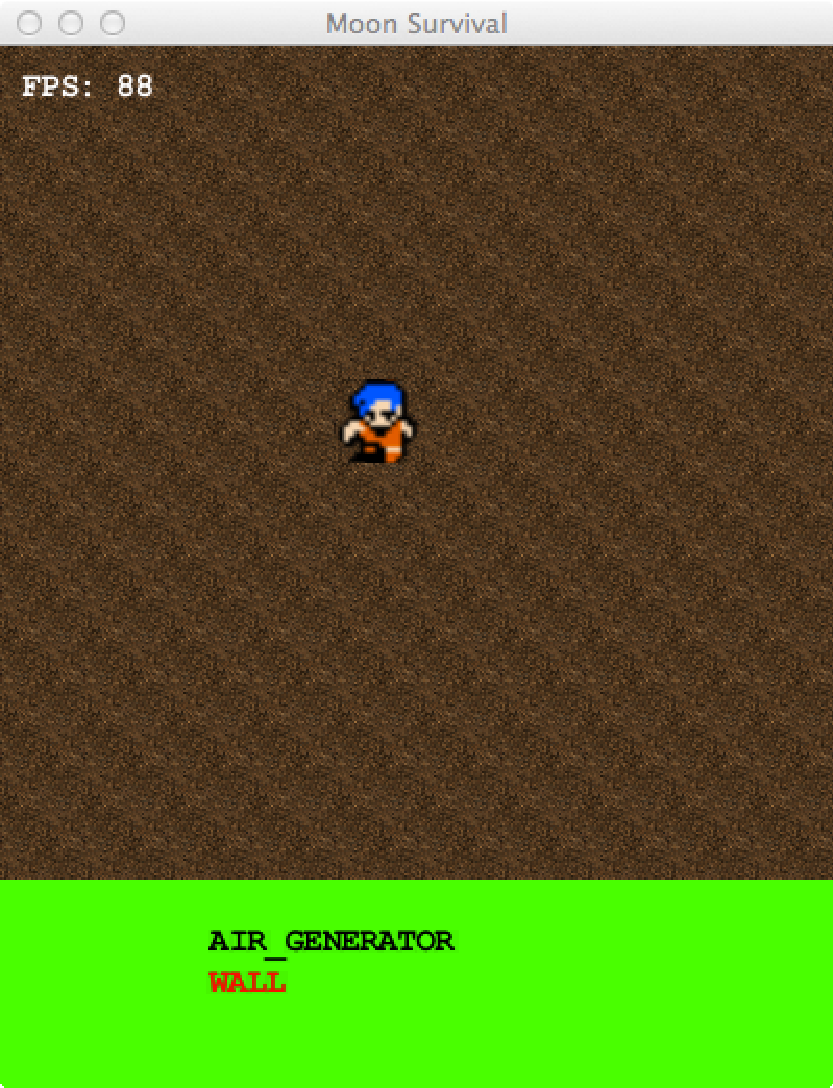
\includegraphics{res/space_base_prototype/no_base.pdf}
	\caption{
	\prototypeSiddall : player on moon with no base
	}
	\label{fig:SpaceBaseNoRoom}
\end{marginfigure}

\begin{marginfigure}
	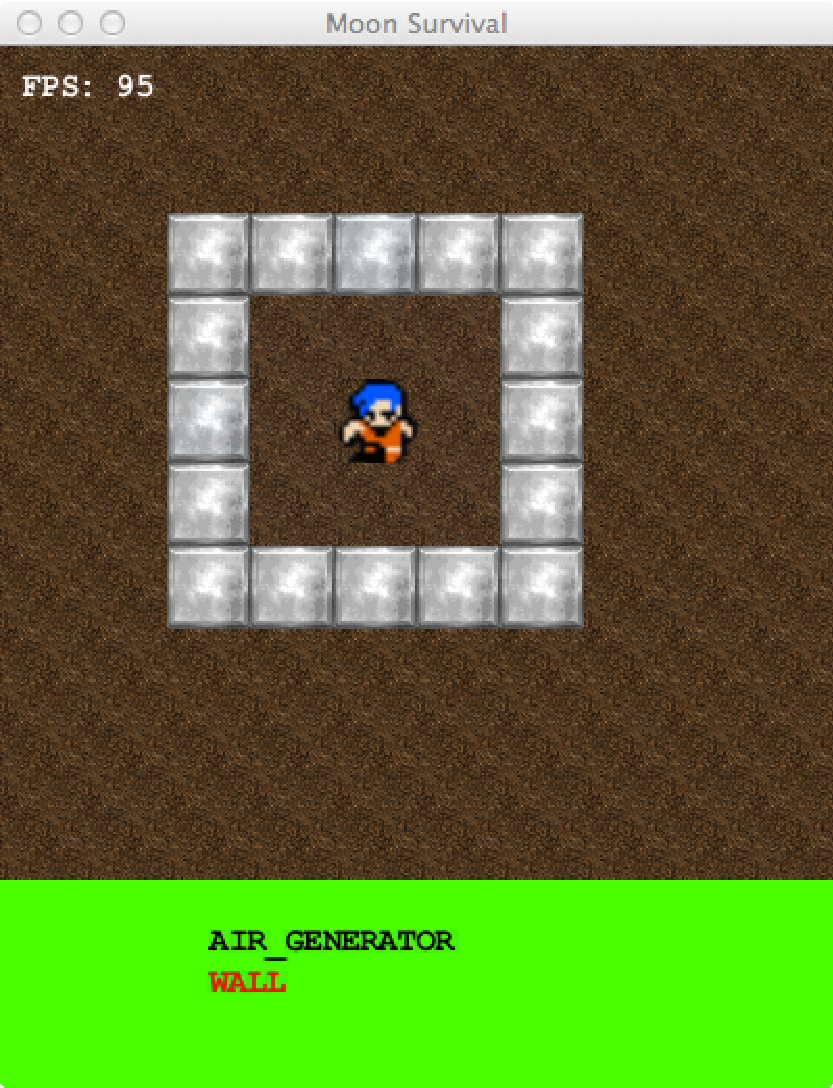
\includegraphics{res/space_base_prototype/empty_room.pdf}
	\caption{
	\prototypeSiddall : walled off room with 5x5 interior	}
	\label{fig:SpaceBaseWithRoom}
\end{marginfigure}

\begin{marginfigure}
	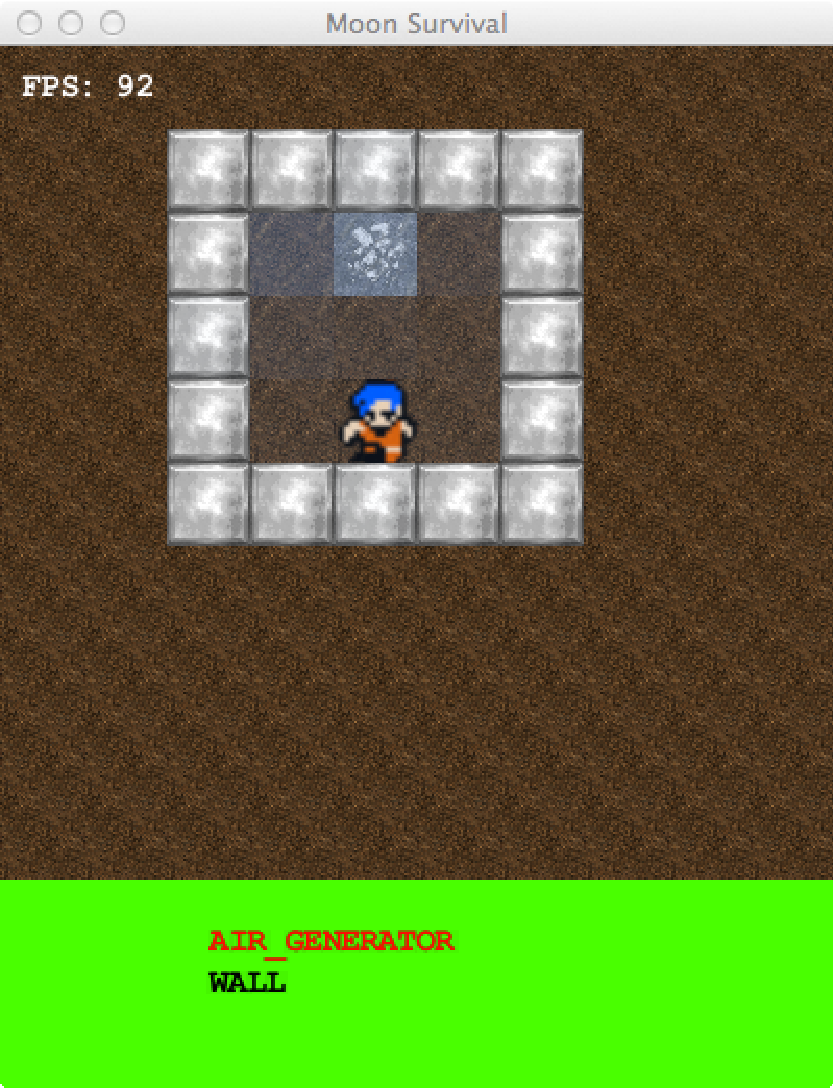
\includegraphics{res/space_base_prototype/room_with_air_generator.pdf}
	\caption{
	\prototypeSiddall : walled off room with 5x5 interior and air generator	}
	\label{fig:SpaceBaseWithAirGenerator}
\end{marginfigure}

\begin{marginfigure}
	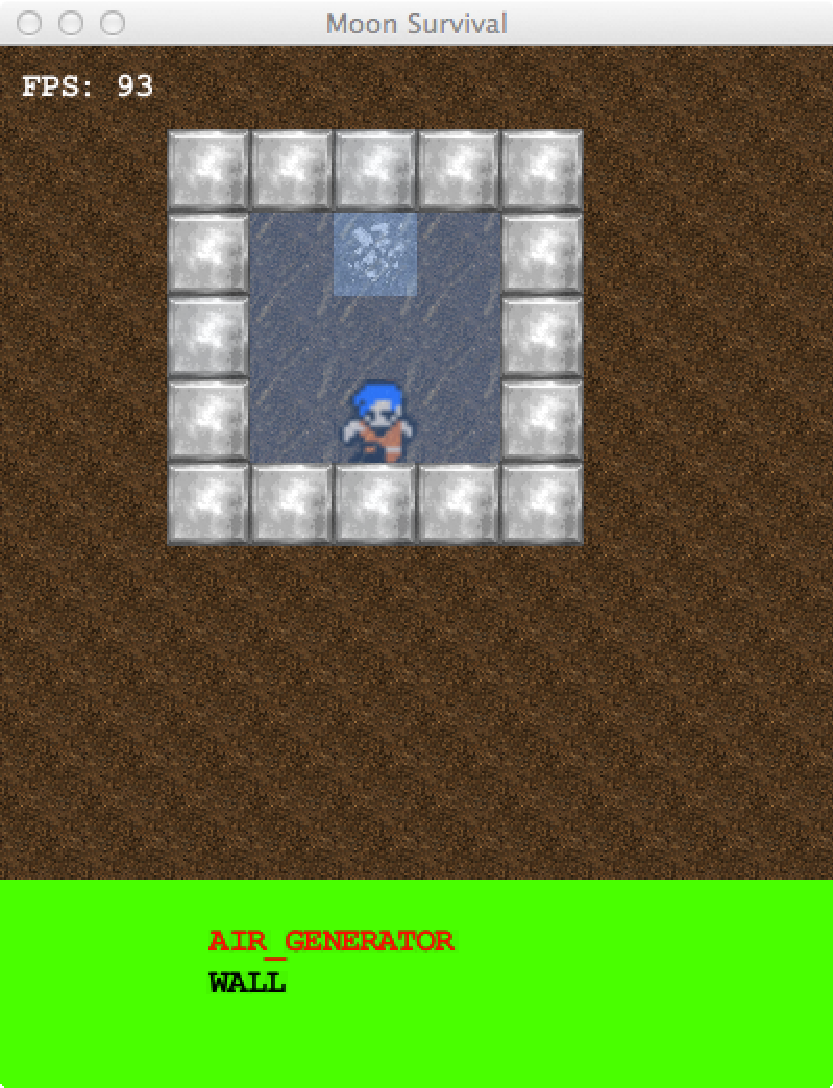
\includegraphics{res/space_base_prototype/room_with_air.pdf}
	\caption{
	\prototypeSiddall : walled off room with 5x5 interior and air	}
	\label{fig:SpaceBaseWithAir}
\end{marginfigure}



In Figure \ref{fig:spaceBaseNoRoom} the player is in a new game with no air and no base.
The player has 2 tools: 
\begin{description}
\item[air generator] makes air and releases it into its immediate surroundings.
\item[wall] solid block that blocks the player walking through it as well as air passing through it.
\end{description}

The first priority is to build a wall around an area so no air can get out.
This is done by placing wall blocks in front of the player.



In Figure \ref{fig:SpaceBaseWithRoom} the Player has now walled of a room.
The next step to place an air generator within the room as shown in Figure \ref. 
This will start generating air. The air will continue to spread until the entire room is filled. 


% game concept
% - building base on moon
% - air
